\documentclass[twocolumn, 12pt]{article}

\usepackage[utf8]{inputenc}
\usepackage[english, spanish]{babel}
\usepackage{fullpage}
\usepackage{graphicx}
\usepackage{amsmath}
\usepackage{enumitem}
\usepackage{chngcntr}
\usepackage{setspace}
\usepackage{url}
\usepackage{csquotes}
\usepackage{float}
\usepackage{verbatim}
\usepackage{tabularx}
\usepackage{amsmath}
\usepackage{caption}
\usepackage{bm}
% \usepackage{hyperref}

\counterwithin{figure}{section}
\renewcommand{\thesection}{\arabic{section}}
\renewcommand{\thesubsection}{\thesection.\arabic{subsection}}
\renewcommand{\baselinestretch}{1.5}

\usepackage[style=apa, maxnames=6, minnames=3, backend=biber]{biblatex}
\DefineBibliographyStrings{english}{%chktex-file 1 chktex-file 6
    andothers = {\em et\addabbrvspace al\adddot}
}
\addbibresource{./Bibliography/bibliography.bib}

\usepackage{array}
\usepackage{enumitem}

\setlength{\parskip}{0pt}

\newcommand{\bolditalic}[1]{\textbf{\textit{#1}}}

\begin{document}

\begin{titlepage}
    \centering
    
\includegraphics[width=0.3\textwidth]{Images/logo_utb.png}\par\vspace{1cm}
    {\scshape\LARGE Universidad Tecnológica de Bolívar \par}
    \vspace{1cm}

    {\scshape\Large FÍSICA CALOR Y ONDAS \par}
    \vspace{.2cm}

    % chktex-file 8
    {\scshape\Large Grupo 1 \par}
    \vspace{1cm}
    % chktex-file 8
    \slshape {\Large \bfseries{}LAB 3 - DIFRACCIÓN DE LA LUZ\\}
    \vspace{4cm}

    \slshape {\itshape{} Mauro González, T00067622 \\}
    % \slshape {\itshape{} German De Armas Castaño, T00068765 \\}
    % \slshape {\itshape{} Angel Vega Rodriguez, T00068186 \\}
    % \slshape {\itshape{} Juan Jose Osorio Ariza, T00067316 \\}
    % \slshape {\itshape{} Jorge Alberto Rueda Salgado, T00068722 \\}
    \vfill
    Revisado Por \\
    Duban Andres Paternina Verona\\
    {\large \today\par}
\end{titlepage}

% ! ----------------------------------------------------------------------|>
\section{Introducción}

La luz, una de las fuerzas fundamentales en el universo, ha
intrigado a científicos y entusiastas de la física a lo
largo de la historia. En particular, uno de los fenómenos
más fascinantes asociados con la luz es la difracción, un
proceso mediante el cual la luz se dobla y se extiende al
pasar por obstáculos o aberturas. La difracción es una
manifestación de la naturaleza ondulatoria de la luz y
puede revelar información valiosa sobre las características
de las ondas luminosas.

En esta experiencia de laboratorio, nos sumergiremos en el
mundo de la difracción de la luz. Utilizaremos una rejilla
de difracción para estudiar este fenómeno y explorar sus
aplicaciones prácticas. A través de esta práctica, no solo
observaremos el comportamiento de la luz cuando pasa por
una estructura en forma de rejilla, sino que también
aprenderemos a calcular la longitud de onda de la luz,
medir el grosor de objetos extremadamente pequeños y
comprender cómo se forman patrones de interferencia.

% ! ----------------------------------------------------------------------|>
\section{Objetivos}

\subsection{Objetivo general}

\begin{itemize}[label=$\triangleright$]
    \item Observar y comprender el fenómeno de difracción de la luz
          utilizando una rejilla de difracción y analizar sus
          aplicaciones.
\end{itemize}

\subsection{Objetivos específicos}

\begin{itemize}[label=$\triangleright$]
    \item Estudiar los principios fundamentales de la difracción de
          la luz, incluyendo el principio de Huygens y la condición
          para obtener un patrón de difracción de Fraunhofer.

    \item Utilizar una rejilla de difracción para calcular la
          longitud de onda de emisión de un láser, aplicando la
          ecuación relacionada con la difracción por una ranura
          simple.

    \item Explorar diferentes configuraciones de rejillas de
          difracción y patrones de difracción, y comprender cómo
          afecta el número de líneas por unidad de longitud a la
          formación de patrones de interferencia.
\end{itemize}

% ! ----------------------------------------------------------------------|>
\section{Preparación de la practica}

% + ------------------------------------------------------------------|>
\subsection{¿Qué es la luz? ¿Cuáles son las características de una luz monocromática?}

Lo que llamamos luz es la parte del espectro
electromagnético que puede ser percibido por el ojo humano.
Existen, aparte de la luz, diversas formas de radiación
electromagnética en el universo, que se propaga por el
espacio y transporta energía de un lugar a otro (como la
radiación ultravioleta o los rayos x), pero a ninguna de
ellas podemos percibirlas
naturalmente.~(\cite{concepto-luz})

La luz monocromática es aquella formada por componentes de
un sólo color. Es decir, es aquella que tiene una única
longitud de onda correspondiente a cada color. Se utiliza,
normalmente, en cámaras monocromáticas. Muy útil para
resaltar algunas características concretas, puesto que cada
color provee mejor visibilidad en ciertos aspectos y
mediante contrastes, ya que todos los colores opuestos se
absorben. A este tipo de luz se le pueden añadir filtros
para separar los anchos de banda o reducir los efectos de
la luz ambiental.~(\cite{concepto-luz-monocromatica})

% + ------------------------------------------------------------------|>
\subsection{¿Qué es la luz? ¿Cuáles son las características de una luz monocromática?}

La propagación de una onda depende del movimiento de su
frente de onda. Conforme avanza el frente de onda, el
movimiento ondulatorio se propaga alcanzando nuevos puntos
del medio.

El principio de Huygens nos permite explicar fenómenos
ondulatorios relacionados con la propagación de la onda,
tales como la reflexión, la refracción y la difracción. Fue
desarrollado en 1678 por Christian Huygens (1629 - 1695),
físico, astrónomo y matemático holandés en su obra
``Tratado de la luz'' y es una descripción geométrica del
fenómeno de la propagación de las ondas a través del
espacio.

Tomado de:~\cite{Fernández}

% + ------------------------------------------------------------------|>
\subsection{¿Qué es la difracción?}

La difracción es un fenómeno que involucra a todas las
ondas: electromagnéticas, de radio, sonoras, etc, y es
posible predecir su desarrollo haciendo uso de distintas
aproximaciones matemáticas. Cuando la onda traspasa una
grieta o se topa con un obstáculo, se
desvía.~(\cite{J_Gardey_2018})

\begin{figure}[H]
    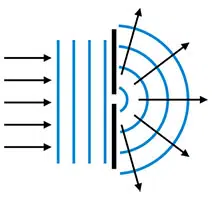
\includegraphics[width=0.9\linewidth]{./Images/Difraccion.jpg}
    \caption{}
\end{figure}

% + ------------------------------------------------------------------|>
\subsection{¿Cuál es la condición para obtener un patrón de difracción de Fraunhofer?}

La condición de Fraunhofer se asegura colocando el
obstáculo en el foco de una lente positiva, permitiendo así
trabajar de forma cómoda con la pantalla a distancia finita
del obstáculo, si bien la observación se realiza a
distancia infinita.~(\cite{Optics})

% + ------------------------------------------------------------------|>
\subsection{Condición de mínimos de intensidad en el patrón de difracción de una sola ranura.}

Los mínimos de intensidad se producen cuando el argumento
del seno es un múltiplo entero de p, es decir, cuando

\begin{equation*}
    \frac{\pi b \sen \theta}{\lambda} = n \pi
\end{equation*}

o bien, cuando

\begin{equation*}
    b \sen \theta = n \lambda (n = 1, 2, 3 \dots)
\end{equation*}

Esta es la fórmula que describe el fenómeno de la
difracción Fraunhofer producido por una rendija estrecha.

Tomado de:~\cite{difraccion}

% + ------------------------------------------------------------------|>
\subsection{¿Cómo se obtiene la longitud de onda de emisión de un láser a través de un montaje de
    difracción por una ranura simple?}

Para obtener la longitud de onda de emisión de un láser a
través de un montaje de difracción por una ranura simple,
se puede utilizar la siguiente fórmula:

\begin{equation*}
    \lambda = a \sin(\theta)
\end{equation*}

Donde $\lambda$ es la longitud de onda, $a$ es el ancho de
la ranura y $\theta$ es el ángulo de difracción.

Es importante tener en cuenta que esta fórmula solo es
aplicable para una ranura simple y no para múltiples
ranuras.

\nocite{Multipleslitdiffraction}

% + ------------------------------------------------------------------|>
\subsection{¿Cómo se obtiene el grosor de un cabello a través de su patrón de difracción?}

La técnica de difracción de Fraunhofer es un método que nos
puede ayudar medir el grosor de un cabello a través de su
patrón de difracción. Al hacer incidir luz láser sobre un
cabello, se produce una imagen de difracción en una
pantalla que es similar a la que se produce en una red de
difracción. La imagen de difracción tiene un máximo central
fuertemente iluminado y máximos secundarios más débiles a
sus lados. La distancia entre el máximo central y el primer
máximo secundario es proporcional al grosor del cabello12.

Para obtener el grosor del cabello, se puede utilizar la
fórmula:

\begin{equation*}
    t = \lambda D / (a \cdot \cos(\theta))
\end{equation*}

Donde $t$ es el grosor del cabello, $\lambda$ es la
longitud de onda del láser, $D$ es la distancia entre la
pantalla y el cabello, $a$ es el ancho de la ranura y
$\theta$ es el ángulo de difracción.

\nocite{optica}

% + ------------------------------------------------------------------|>
\subsection{Registrar datos en una tabla}

\begin{table}[H]
    % chktex-file 44
    \begin{center}
        \begin{tabularx}{0.9\linewidth}{|>{\centering\arraybackslash}X|>{\centering\arraybackslash}X|}
            \hline
            Lineas/mm                     & 1 \bolditalic{linea/mm} \\\hline
            Longitud de onda              & 632.8 \bolditalic{nm}   \\\hline
            Distancia de observación      & 100 \bolditalic{cm}     \\\hline
            Posición de máximos o mínimos & 0.0633 \bolditalic{cm}  \\\hline
        \end{tabularx}
    \end{center}
\end{table}

\vspace{-.5cm}

\begin{table}[H]
    % chktex-file 44
    \begin{center}
        \begin{tabularx}{0.9\linewidth}{|>{\centering\arraybackslash}X|>{\centering\arraybackslash}X|}
            \hline
            Lineas/mm                     & 5 \bolditalic{linea/mm} \\\hline
            Longitud de onda              & 632.8 \bolditalic{nm}   \\\hline
            Distancia de observación      & 100 \bolditalic{cm}     \\\hline
            Posición de máximos o mínimos & 0.3164 \bolditalic{cm}  \\\hline
        \end{tabularx}
    \end{center}
\end{table}

\vspace{-.5cm}

\begin{table}[H]
    % chktex-file 44
    \begin{center}
        \begin{tabularx}{0.9\linewidth}{|>{\centering\arraybackslash}X|>{\centering\arraybackslash}X|}
            \hline
            Lineas/mm                     & 10 \bolditalic{linea/mm} \\\hline
            Longitud de onda              & 632.8 \bolditalic{nm}    \\\hline
            Distancia de observación      & 100 \bolditalic{cm}      \\\hline
            Posición de máximos o mínimos & 0.6328 \bolditalic{cm}   \\\hline
        \end{tabularx}
    \end{center}
\end{table}

\vspace{-.5cm}

\begin{table}[H]
    % chktex-file 44
    \begin{center}
        \begin{tabularx}{0.9\linewidth}{|>{\centering\arraybackslash}X|>{\centering\arraybackslash}X|}
            \hline
            Lineas/mm                     & 15 \bolditalic{linea/mm} \\\hline
            Longitud de onda              & 632.8 \bolditalic{nm}    \\\hline
            Distancia de observación      & 100 \bolditalic{cm}      \\\hline
            Posición de máximos o mínimos & 0.9492 \bolditalic{cm}   \\\hline
        \end{tabularx}
    \end{center}
\end{table}

\nocite{Diffractiongrating}

% ! ----------------------------------------------------------------------|>
\section{Resumen del procedimiento}

En esta experiencia de laboratorio, se busca observar y
comprender el fenómeno de difracción de la luz a través de
la utilización de un láser y una rejilla de difracción. El
procedimiento se divide en varios pasos:

\begin{enumerate}
    \item \textbf{Configuración Inicial}: El láser de semiconductor se coloca
          sobre una base de soporte en un extremo del riel. Se coloca
          una pantalla cerca de la salida del láser.

    \item \textbf{Alineación del Láser}: Se enciende el láser y se marca el
          punto en la pantalla donde incide el haz láser. Luego, se
          retira la pantalla hacia el otro extremo del riel y se
          ajusta la dirección del láser para que incida nuevamente en
          el punto marcado. Esto asegura que el láser esté alineado
          adecuadamente.

    \item \textbf{Preparación de la Red de Difracción}: Se coloca la red de
          difracción en una base de soporte frente a la salida del
          láser.

    \item \textbf{Alineación de la Red de Difracción}: Se enciende el láser y
          se ajusta la altura de la rejilla de difracción hasta que
          el haz láser incida en el centro de la rejilla, generando
          un patrón de difracción en la pantalla.

    \item \textbf{Medición de Distancias}: Se mide la distancia $(D)$ entre la
          red de difracción y la pantalla de observación. Además, se
          registran las posiciones de los tres primeros máximos en el
          patrón de difracción observado en la tabla.

    \item \textbf{Cambios en el Ancho de la Ranura}: El procedimiento se
          repite con diferentes valores de $D$, que representan
          diferentes anchos de la ranura, y se registra la posición
          de los máximos correspondientes en cada caso.

    \item \textbf{Difracción por un Cabello}: En lugar de la red de
          difracción, se coloca un cabello frente al láser. Se
          registran las posiciones de los tres primeros mínimos en el
          patrón de difracción y se mide la distancia desde el
          cabello hasta la pantalla.

    \item \textbf{Medición del Grosor del Cabello}: Se utiliza un calibrador
          micrométrico para medir el grosor del cabello.
\end{enumerate}

Este procedimiento permite la observación directa de los
efectos de la difracción de la luz y proporciona datos
experimentales para el análisis. Se estudian tanto los
patrones de difracción generados por una rejilla como por
un cabello, lo que permitirá comprender los principios de
la difracción y su aplicación en la medición de propiedades
microscópicas, como el grosor de un cabello.

\printbibliography

\end{document}